\documentclass[12pt,a4paper,titlepage]{article}
\usepackage[utf8]{inputenc}
\usepackage{polski}
\usepackage{listings}
\usepackage{graphicx}
\usepackage{xcolor}
\usepackage{minted}
\usepackage{amsmath}
\usepackage{caption}
 
\setminted{
    linenos=true,
    autogobble,
    breaklines,
    frame=lines,
    framerule=1pt,
    framesep=10pt
}

\newenvironment{longlisting}{}{}

\makeatletter
\newcommand{\linia}{\rule{\linewidth}{0.4mm}}
\renewcommand{\maketitle}{\begin{titlepage}
    \vspace*{1cm}
    \begin{center}\small
    Politechnika Wrocławska\\
    Wydział Elektroniki\\
    Grafika Komputerowa i Komunikacja Człowiek-Komputer
    \end{center}
    \vspace{3cm}
    \noindent\linia
    \begin{center}
      \LARGE \textsc{\@title}
         \end{center}
     \linia
    \vspace{0.5cm}
    \begin{flushright}
    \begin{minipage}{7cm}
    \textit{\small Autor:}\\
    \normalsize \textsc{\@author} \par
    \end{minipage}
    \vspace{5cm}

     {\small czwartek, 17\textsuperscript{15}-20\textsuperscript{15} TN}\\
        mgr inż. Szymon Datko
     \end{flushright}
    \vspace*{\stretch{6}}
    \begin{center}
    \@date
    \end{center}
  \end{titlepage}%
}
\makeatother
\author{Justyna Skalska, 225942}
\title{Sprawozdanie nr 5\\
(OpenGL - teksturowanie powierzchni obiektów)}

\begin{document}

\maketitle
\section{Omówienie tematu}
Naszym zadaniem na laboratorium było stworzenie prostego programu wprowadzającego do teksturowania obiektów w scenach 3D z wykorzystaniem OpenGL wraz z rozszerzeniem GLUT. Głównym zadaniem było oteksturowanie jajka używając własnej tekstury zapisanej w formacie TGA. Obrazek miał znajdować się po obu stronach jajka i być dopasowanym do jego wysokości oraz szerokości.

\begin{figure}[H]
\centering

\includegraphics[width = 9cm]{images/tekstura.png}
\caption{Tekstura nałożona na jajko}
\label{fig:tekstura}
\end{figure}

Tekstura to obraz jedno-, dwu- lub nawet trójwymiarowy wykorzystywany do dodania obiektowi detali. W wersji 1.3 biblioteki OpenGL dodano także tekstury sześcienne. W ćwiczeniu wykorzystywaliśmy tylko tekstury dwuwymiarowe. Współrzędne tekstury leżą w zakresie od 0 do 1 na osiach X i Y (dla tekstur 2D). Pobranie koloru tekstury przy użyciu koordynat nazywa się próbkowaniem (ang. sampling). Współrzędne tekstury zaczynają się w punkcie (0,0) od lewego dolnego rogu obrazka do punktu (1,1) dla prawego górnego rogu. Teksturowanie jest dostępne tylko w trybie RGB(A).

\begin{figure}[H]
\centering
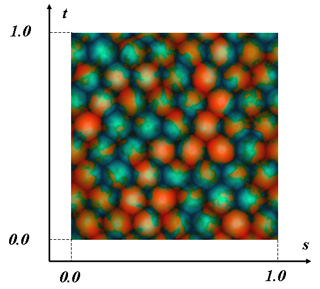
\includegraphics[width = 9cm]{images/coordinates.jpg}
\caption{Wzorzec w układzie współrzędnych tekstury}
\label{fig:koordynaty}
\end{figure}

\section{Omówienie kodu}

\begin{listing}[H]
\caption{Funkcja zwracająca współrzędne tekstury}
\begin{minted}{C++}
Point** getTextures(int n) {
  // stworzenie dwuwymiarowej tablicy współrzędnych tekstury
  Point** textures = new Point*[n + 1];
  for (size_t i = 0; i < n + 1; i++) {
    textures[i] = new Point[n + 1];
  }

  for (size_t i = 0; i < n + 1; i++) {
    for (size_t j = 0; j < n + 1; j++) {
      double u = (double)i / (double)n;
      double v = (double)j / (double)n;

      // zapewnienie poprawnego nakładania tekstury dla obu połówek jajka
      if (i > (n / 2) - 1) {
        textures[i][j].x = v;
        textures[i][j].y = 1 - fmod(2 * u, 1.0);
      } else {
        textures[i][j].x = v;
        textures[i][j].y = fmod(2 * u, 1.0);
      }
    }
  }

  return textures;
}
\end{minted}
\end{listing}

\newpage
\begin{longlisting}
\begin{minted}{C++}
void drawEggFromTriangles(int n, Point** bezierValues, Point** normals, Point** textures) {

  glBegin(GL_TRIANGLES);
  
  for (size_t i = 0; i < n; i++) {
    for (size_t j = 0; j < n; j++) {
      // podanie punktów współrzędnych tekstury potrzebnych do nałożenia jej na jajko
      glTexCoord2f(textures[i][j].x, textures[i][j].y);
      glNormal3f(normals[i][j].x, normals[i][j].y, normals[i][j].z);
      glVertex3f(bezierValues[i][j].x, bezierValues[i][j].y - 5, bezierValues[i][j].z);

      glTexCoord2f(textures[i + 1][j].x, textures[i + 1][j].y);
      glNormal3f(normals[i + 1][j].x, normals[i + 1][j].y, normals[i + 1][j].z);
      glVertex3f(bezierValues[i + 1][j].x, bezierValues[i + 1][j].y - 5, bezierValues[i + 1][j].z);

      glTexCoord2f(textures[i + 1][j + 1].x, textures[i + 1][j + 1].y);
      glNormal3f(normals[i + 1][j + 1].x, normals[i + 1][j + 1].y, normals[i + 1][j + 1].z);
      glVertex3f(bezierValues[i + 1][j + 1].x, bezierValues[i + 1][j + 1].y - 5, bezierValues[i + 1][j + 1].z);

      glTexCoord2f(textures[i][j + 1].x, textures[i][j + 1].y);
      glNormal3f(normals[i][j + 1].x, normals[i][j + 1].y, normals[i][j + 1].z);
      glVertex3f(bezierValues[i][j + 1].x, bezierValues[i][j + 1].y - 5, bezierValues[i][j + 1].z);

      glTexCoord2f(textures[i][j].x, textures[i][j].y);
      glNormal3f(normals[i][j].x, normals[i][j].y, normals[i][j].z);
      glVertex3f(bezierValues[i][j].x, bezierValues[i][j].y - 5, bezierValues[i][j].z);

      glTexCoord2f(textures[i + 1][j + 1].x, textures[i + 1][j + 1].y);
      glNormal3f(normals[i + 1][j + 1].x, normals[i + 1][j + 1].y, normals[i + 1][j + 1].z);
      glVertex3f(bezierValues[i + 1][j + 1].x, bezierValues[i + 1][j + 1].y - 5, bezierValues[i + 1][j + 1].z);
    }
  }
  
  glEnd();
}
\end{minted}
\end{longlisting}
\begin{listing}
\caption{Funkcja rysujący jajko z teksturą}
\end{listing}

\section{Rezultat prac}
Udało mi się wykonać wszystkie podpunkty zadania. Wybrana tekstura została przeze mnie nałożona na obie połówki jajka, a obrazek został dopasowany do jego szerokości oraz wysokości. Scena została także oświetlona dwoma źródłami światła, jednym - czerwonym, drugim - niebieskim. Obiekt obracał się wokół własnej osi po nieciśnięciu lewego przycisku myszy.

\begin{figure}[H]
\centering
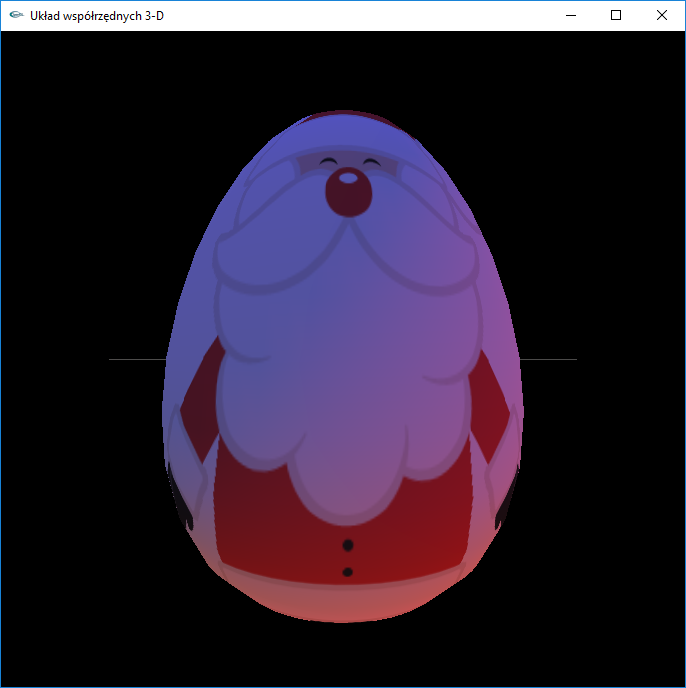
\includegraphics[width = 9cm]{images/santa.png}
\caption{Przód jajka z nałożoną teksturą}
\label{fig:mikolaj_przod}
\end{figure}

\begin{figure}[H]
\centering
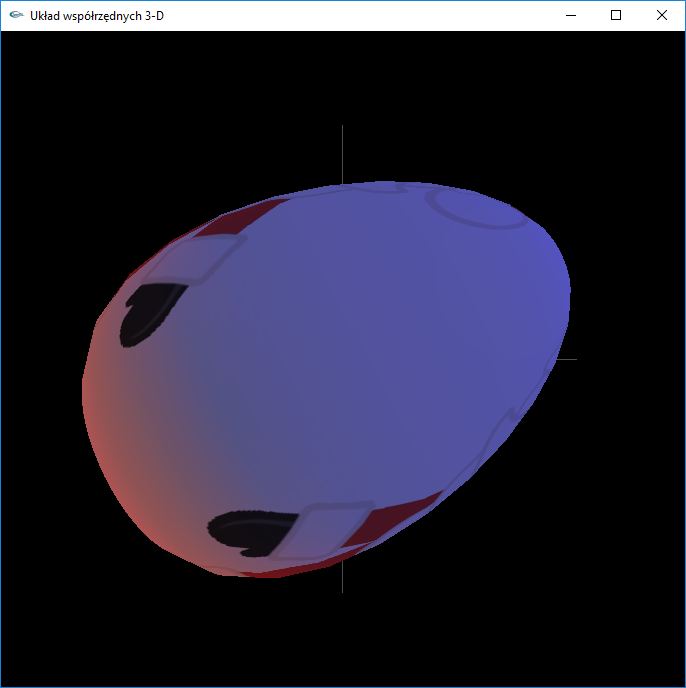
\includegraphics[width = 9cm]{images/santa1.png}
\caption{Tekstura na łączeniu połówek jajka}
\label{fig:mikolaj_bok}
\end{figure}

\end{document}
